\documentclass[10pt,twocolumn]{article}
\usepackage[a4paper,margin=1.9cm,columnsep=0.7cm]{geometry}
\usepackage{mathptmx}
\usepackage[T1]{fontenc}
\usepackage{microtype}
\usepackage{graphicx}
\usepackage{booktabs}
\usepackage{array}
\usepackage{caption}
\usepackage{authblk}
\usepackage[hidelinks]{hyperref}
\usepackage{xcolor}

\captionsetup{font=small,labelfont=bf,skip=5pt}
\raggedbottom
\setlength{\parindent}{1.1em}
\definecolor{mono}{HTML}{2F6F9F}
\definecolor{dia}{HTML}{C25A3C}

\title{\vspace{-1.2em}\bfseries Monologue or Dialogue?\\[2pt]
\large Measuring Conversational Structure in the Reasoning Traces of Large Language Models}
\author[ ]{Oskar Engl}
\affil[ ]{\small Johannes Kepler University Linz, Austria}
\affil[ ]{\small \textit{oskar.engl@ik.me}}
\date{\small Working version, July 2026}

\begin{document}
\twocolumn[
\begin{@twocolumnfalse}
\maketitle
\begin{abstract}
\noindent
Reasoning models such as DeepSeek-R1 produce a long stretch of intermediate tokens before they
answer. Although each stretch is written by a single model in one pass, one can observe in a trace
that questions receive answers, objections receive concessions, and the argument turns against
itself and starts again. Is a reasoning trace's textual shape more akin to a monologue or to a
dialogue? We examine this with three text-analysis methods, two from stylometry and one from
conversation analysis, and require each to prove itself first on four corpora whose voice structure
is known: human monologue, human dialogue, AI monologue and AI dialogue. Only a method that
separates monologue from dialogue on these known datasets goes on to measure the traces. Two of the
three do. Both place the DeepSeek-R1 traces above the four-instance AI debate on their own measure:
the traces change style between neighbouring sentences more often than the debate does, and they
complete more question-and-answer pairs than the debate, though several times fewer than a single
person thinking aloud. The observed text alone cannot settle whether that comes from several voices
or from one voice writing conversationally.
\medskip
\end{abstract}
\end{@twocolumnfalse}
]

\begin{figure*}[t]
\centering
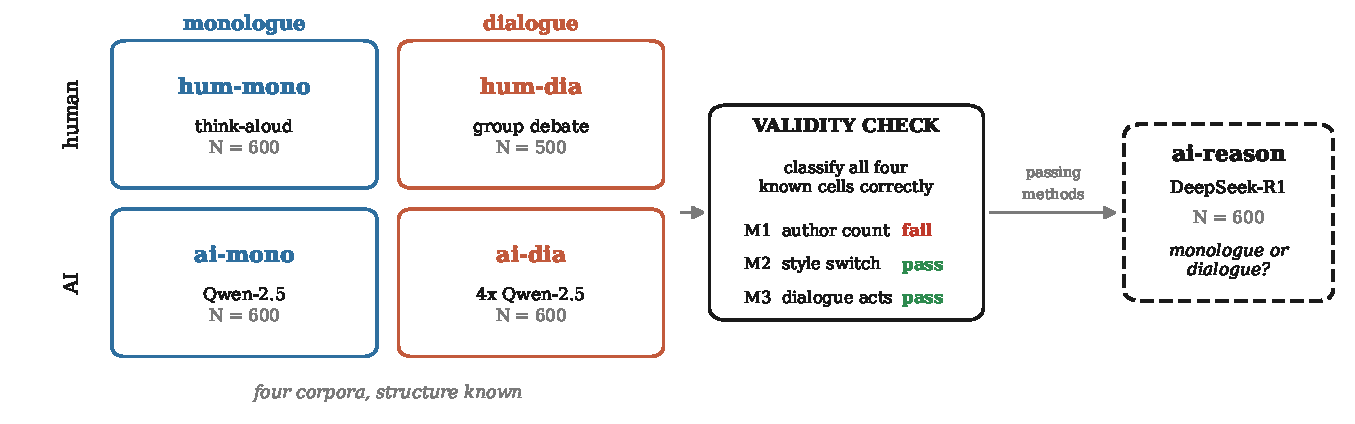
\includegraphics[width=0.96\textwidth]{figures/fig_grid.pdf}
\caption{\textbf{Study design.} Four corpora of known voice structure (left) supply the validity
check: a method goes forward only if it sorts the four known cells correctly into monologue and
dialogue. Two of the three methods do so. The passing methods then measure the DeepSeek-R1
reasoning traces (\texttt{ai-reason}). The results report all four known cells alongside the traces;
the two AI cells carry the most weight, because they share both their producer and their
task with the traces, while the human cells differ in producer, and we read them with that in mind.}
\label{fig:grid}
\end{figure*}

\section{Introduction}
Reasoning-oriented training has become standard in frontier models. Given a problem, a model such as
DeepSeek-R1 \cite{guo2025} first produces a long stretch of intermediate tokens
\cite{kambhampati2025}, commonly called a reasoning trace, and only then gives its final answer.
These traces have a notable feature: a single model writes each one in one pass, yet a trace often
contains questions and their answers, objections and concessions, and sudden reversals of direction.
In writing by people, features like these can mark a real exchange between participants. But they can
equally mark the deliberation of a single voice.

Kim et al.~\cite{kim2026} argue that reasoning-trained models improve in part because they simulate
a ``society of thought,'' a set of internal perspectives that propose, criticise, and reconcile.
Cognitive science offers older parallels: it has understood reasoning as a social and
argumentative activity \cite{mercier2017} and the mind as a set of interacting agents
\cite{minsky1986}. Together with the surface features just described, this raises the question we
take up here: is a reasoning trace's textual shape more akin to a monologue or to a dialogue?

Our study rests on one assumption: if several separate voices take turns in a trace, the structure of
the writing should show it. Authorship research has found that writers
differ in small, largely involuntary habits, most robustly in how they use function words, and that
these habits are stable within an author and vary between authors \cite{stamatatos2009}. We
therefore restate the question so that a text-analysis method can answer it: a monologue should read
as the work of one author and a dialogue as the work of several, so we ask which of the two the
traces are closer to.

\section{Design}
Reasoning-trained models have been widely available only since 2025 \cite{guo2025}, so there is
little prior work on the voice structure of their traces. We therefore compare against a grid
of corpora whose structure \emph{is} known (Figure~\ref{fig:grid}).

\textbf{Four known corpora, and the target.} We vary two properties across the grid: who produced
the text (a human or an AI) and whether it is a monologue or a dialogue. The four cells are human
monologue (think-aloud protocols, in which a person speaks their thoughts aloud while solving a task
\cite{wurgaft2025}; $N=600$), human dialogue (group deliberation from DeliData \cite{karadzhov2023};
$N=500$), AI monologue (a single Qwen-2.5-7B model solving a puzzle on its own; $N=600$), and AI
dialogue (four separate copies of Qwen-2.5-7B, each given a role, taking turns in a debate;
$N=600$). The fifth cell is DeepSeek-R1: we give the model the same puzzle and take its
native thinking trace, the reasoning it produces before its final answer, as the document ($N=600$).
This is the cell whose structure we want to determine.

\textbf{The validity check.} Performance on the grid earns a method the right to judge the traces.
We define the check at the level of the cell and apply it to every method: a method is carried
forward only if it sorts the four known cells correctly into monologue and dialogue.

\textbf{Holding the task fixed.} The AI monologue, AI dialogue, and AI reasoning cells all solve the
same puzzle, Game of 24 \cite{yao2023}, in which four given numbers must be combined with the four
basic arithmetic operations to reach 24, and so does the human monologue cell. This
rules out a method separating the cells by their subject matter rather than by their voice structure.
The puzzle also sits near the limit of the Qwen model's ability, so the two AI corpora contain
genuine problem-solving rather than instant recall or uniform failure. The human dialogue cell is the
one exception, since it uses the Wason card task, another compact logic puzzle, because no
group-deliberation corpus exists for Game of 24. Producer and task are therefore constant only across
the three AI cells, so those two AI cells carry the most weight in the comparisons and the human
cells stand beside them as reference points. We also removed the speaker labels from both dialogue corpora, so that the
corpora differ as little as possible apart from the number of speakers producing the text.

\section{Methods}
The three methods read different signals, so that agreement among them carries more weight than a
single method alone. Each yields a measurement per document, which we summarise per cell and read as
pointing towards monologue or towards dialogue.

\textbf{Method 1: counting authors across the document} \cite{nath2019}. This was the top-ranked
system in the PAN 2019 style change detection task, at $84.8\%$ accuracy on the binary single against
multi-author decision \cite{zangerle2019}. It divides a document into paragraph-sized windows,
describes each window by how often the 50 most common words occur in it, and groups similar windows
together. It reads the number of groups as the number of authors, which we reduce to a binary
decision: one author (monologue) or more than one (dialogue). A cell counts as correctly classified
if most of its documents fall on the right side of that decision.

\textbf{Method 2: detecting style changes between sentences} \cite{schmidt2025}. This method
works sentence by sentence, splitting documents with the Punkt tokenizer. For each pair of
neighbouring sentences it estimates the probability that the two were written by different authors,
using an encoder trained to capture writing style while ignoring topic \cite{patel2025}. Averaging
those probabilities over a document gives its score: the mean probability that any two adjacent
sentences were written by different people.

That score falls as documents get longer (Figure~\ref{fig:split}A). The decline holds in all four
known corpora, steeply in the
two monologue cells and mildly in the human debate, but not in the reasoning traces, whose score is
nearly flat from $72$ to $959$ sentence pairs. Since the corpora differ greatly in typical length,
comparing them directly would measure length as much as structure. We handle this by comparing like
with like: each document in one cell is compared only against documents in the other whose length is
within five percent of its own. We then report the mean difference in score, and the share of
documents that scored above their matches. Two cells can be compared this way
only where their lengths overlap, and we report below where that condition fails.

\textbf{Method 3: measuring question-and-answer structure} \cite{schegloff1973}. This method reads
the text as a sequence of conversational moves. Tencent Hunyuan Hy3, a mixture-of-experts model with
295B parameters of which 21B are active per token, tags each utterance with its function using CAMS
\cite{duran2022}, a standard scheme whose 27 labels include tags such as
\texttt{propositionalQuestion}, \texttt{answer} and \texttt{inform}. The signal we specified in
advance for classification is how often the text completes an \emph{adjacency pair}. An adjacency pair is the basic
sequential unit of conversation, a two-part exchange in which the first part makes a specific second
part due, such as a question followed by an answer, or a proposal followed by its acceptance; it is
the mechanism that binds one participant's turn to another's \cite{schegloff1973}. A single writer can produce completed pairs as well, and think-aloud
protocols do so often, so the rate carries information only against a comparable baseline. We
therefore validate the method by checking that within each producer the dialogue documents complete
pairs at a higher rate than their monologue counterpart.

\textbf{Deviation from the pre-registered gates.} We originally pre-registered a separate statistical
gate for each method, rather than the single check we use here. Under those gates Method~1 would have
passed, and Method~3 was blocked by a label-reliability threshold ($\kappa \ge 0.70$, discussed in
Section~4.1). This was a problem: the gates admitted a method that reads most debates as the work of
a single author, and excluded a method that correctly separates all four known cells. We therefore
report against a method's ability to tell the monologue cells from the dialogue cells in the four
known corpora, applied identically to all three methods.

\section{Results}

\subsection{Which methods qualify}
Two of the three methods, Method~2 and Method~3, sort all four known cells correctly and are carried
forward to give their judgment on the reasoning traces. Method~1 misclassifies both dialogue cells.

\textbf{Method 1 fails the check.} On single-author text the method correctly labels $97.5\%$ of the
human monologue documents and $99.8\%$ of the AI monologue documents. On
multi-author text it collapses: it recovers $42.3\%$ of the AI debates, so a majority of four-way
debates are read as the work of one author, and \emph{none} of the human debates, calling all $500$
of them single-author. It therefore places both known dialogue cells on the monologue side.

The human deliberation corpus we used likely explains the result. DeliData's turns average $8.4$
words, with a median of $6$, against $166$ words per turn in the AI debate. Method~1 describes
paragraph-sized windows by their function-word profile, and at six words per turn a single window
absorbs several speakers at once, leaving little for the clustering to separate.
Table~\ref{tab:verdict} records its reading of the traces for completeness.

\textbf{Method 2 passes.} Because the corpora vary greatly in length, and because length influences
this score, we compare each debate document only against monologue documents of near-identical
length. Compared this way, both producer pairs separate in the right direction. Human debate
documents score $+0.0434$ above their length-matched think-aloud counterparts (95\% CI
$[+0.0375,+0.0495]$), and $72\%$ of them exceed their monologue match in style switching. AI debates score $+0.0232$
above their length-matched AI monologues (95\% CI $[+0.0205,+0.0260]$), with $80\%$ exceeding their
monologue match. The separation is therefore not an artifact of the two cells differing in length: it
holds when length is held equal.

\textbf{Method 3 passes, with a caveat about its labels.} Its completion rate separates dialogue from
monologue in the expected direction within each producer, $0.235$ against $0.095$ for the human cells
and $0.025$ against $0.003$ for the AI cells, with Cliff's $\delta=0.4717$.

These numbers rest on labels from an automatic tagger, so we measured that tagger against a
human annotator on $503$ utterances. The two chose the same label in $74.2\%$ of cases, giving
Cohen's $\kappa=0.54$, or $0.62$ under the tree-weighted coefficient the CAMS authors recommend
\cite{duran2022}. Either way this falls short of the $\kappa\ge0.70$ we had pre-registered. Most
disagreements are near misses of one kind, $101$ of $130$ turning on the general \texttt{inform}
label against a more specific one that also fits, and they split evenly in both directions. Labelling
every utterance correctly and separating the cells are two different achievements, and the check
establishes only the second; we carry Method~3 forward on that basis and treat its labels as the
weakest link in its chain, with further checks planned (Section~7).

\begin{figure*}[t]
\centering
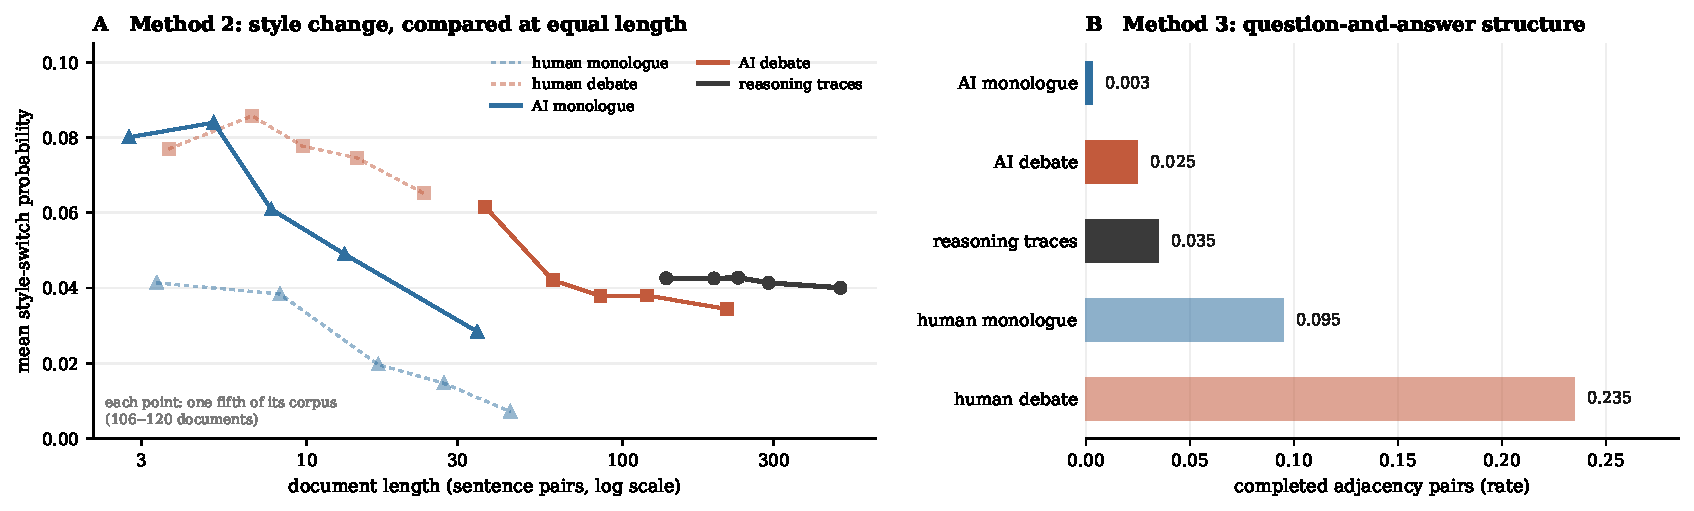
\includegraphics[width=0.98\textwidth]{figures/fig_split.pdf}
\caption{\textbf{What each passing method measures.} (A) Method~2: mean probability that two
adjacent sentences were written by different authors, against document length. Every cell's score
falls with length, which is why we compare cells only at equal length; the reasoning traces are the
one cell that stays flat. Where the traces and the AI debate overlap, the traces sit above. The other
three cells reach no trace length, but both monologue cells are already below the traces at their own
longest documents, while the human debate is still above its own; this is why we can bound the traces
against the monologue cells and not place them against the human debate. Points are binned for
display only: we split each cell into five equal-count (quantile-spaced) length bins, following the
standard recommendation for binned scatter plots \cite{cattaneo2024binscatter}, so every point rests
on the same number of documents (106--120) and no minimum-count threshold is imposed. The statistics
in Section~4 use length-matched documents and no bins. (B) Method~3: rate of completed adjacency pairs per cell. The traces exceed the AI debate
but fall several times below a single person thinking aloud.}
\label{fig:split}
\end{figure*}

\begin{table}[t]
\centering
\small
\setlength{\tabcolsep}{3.5pt}
\caption{The three methods against the validity check, and where each places the traces. We bracket
Method~1's reading, since it fails the check and so does not judge them. Figure~\ref{fig:split}
gives the values behind these readings.}
\label{tab:verdict}
\begin{tabular}{@{}lc>{\raggedright\arraybackslash}p{3.85cm}@{}}
\toprule
Method & Passes & Reading of the traces \\
\midrule
1: author count & no & [between AI monologue and AI debate] \\
2: style switch & yes & more switches than AI debate \\
3: adjacency pairs & yes & more pairs than AI debate, fewer than human \\
\bottomrule
\end{tabular}
\end{table}

\subsection{What the surviving methods report}
Both methods place the reasoning traces above the AI debate. Figure~\ref{fig:split} shows each
method on its own measure, and inspecting it helps in understanding the analysis below.

\textbf{Method 2 (switch probability, Figure~\ref{fig:split}A).} Compared against AI debate documents
of the same length, the reasoning traces score $+0.0109$ higher (95\% CI $[+0.0099,+0.0119]$), and
$85\%$ of traces score above the debate documents nearest to them in length. These $540$ comparisons
draw on $375$ distinct debate documents, so the result does not rest on a few reused matches.

The remaining three cells cannot be length-matched to the traces directly. Only eight AI monologue
documents are long enough to match any trace, and the human cells are shorter still and do not
overlap with the traces at all. For the two monologue cells a weaker comparison is still possible.
Switch probability falls with length, and the traces are the longest corpus in the study, so we read
the traces at the lengths where this measure runs lowest; even so, their switch
probability stays between $0.040$ and $0.043$ across their whole range. Both monologue cells sit
below that at their own longest documents: $0.007$ for the human monologue (longest fifth, $34$--$75$
pairs) and $0.028$ for the AI monologue (longest fifth, $19$--$209$ pairs). For either to reach the
traces, its downward trend with length would have to reverse and raise its score by a factor of
$5.6$ for the human monologue and $1.4$ for the AI monologue. We read the human monologue comparison as
secure on this basis and the AI monologue comparison as suggestive; the latter's margin is narrow
enough that a modest upturn would close it.

The human debate is a different case, since it sits \emph{above} the traces throughout its range
($0.065$, across $17$--$50$ pairs). Placing the traces against it would need its decline to continue
well past the longest human debate on record, and the data cannot speak on that. Method~2
therefore leaves the traces unplaced against the human debate.

\textbf{Method 3 (adjacency-pair completion, Figure~\ref{fig:split}B).} The traces complete pairs at $0.035$, above the AI
debate's $0.025$ and well above the AI monologue's $0.003$. The human cells change the picture: a
single person thinking aloud reaches $0.095$ and human debate $0.235$. On this measure, which tracks
conversational moves most directly, the traces sit at roughly a third of one person's self-talk and a
seventh of real conversation.

\section{Discussion}
The traces change more in style than the AI debate does, and complete adjacency pairs at a rate above
the AI debate but far below a person thinking aloud. Both statements are about the writing: the
methods read the text a model produced, and not the computation that produced it.

\textbf{The scope of the claim.} A dialogic reading admits several explanations, and this design
separates only some of them. A trace may be self-talk, one voice posing questions and answering them.
It may be one producer composing an exchange deliberately, as a novelist writes dialogue between
several characters. Or it may be several producers taking turns, as in the human debate cell. The
grid anchors the first and the third: think-aloud is self-talk, and the human debate and the four
role-prompted instances are several producers. It holds no instance of the second. The measurements
can therefore place the traces against self-talk and against multi-producer exchange, and they cannot
separate one producer composing an exchange from several producers holding one. Against the AI
corpora the result leans in the direction Kim et al.~\cite{kim2026} describe; against people, the
measure that tracks conversational moves puts the traces well short of conversation.

\textbf{One voice can adopt a conversational register.} The competing account is that a single
generator has learned to write in a self-questioning register. DeepSeek-R1 was trained on
outcome-based rewards, and its authors report that reflective re-evaluation emerged without being
targeted directly \cite{guo2025}. The two methods are exposed to that account unequally. Method~3 is
the more exposed of the two: a single writer can pose questions and answer them, and think-aloud
does so at nearly four times the AI debate's rate. One reading of the traces' position, above the AI
debate but far below think-aloud, is that reasoning training moves the model some way toward the
pattern of a person thinking aloud, which is a form of self-talk rather than evidence of several
voices.

Method~2 is exposed more narrowly, because it keys on features writers do not control
deliberately, and it can establish that neighbouring sentences read as the work of different
authors. What it cannot establish is whether that comes from several persistent voices or from one
generator whose register and style move as its approach moves, without the voices being uniquely
distinguishable and repeating.

\textbf{How much the AI debate anchor can carry.} Both methods place the traces past that anchor, so
it deserves scrutiny before we take the distance at face value. Its four voices are four instances
of one model distinguished by role prompt. That limits how far apart their writing habits can drift,
and it also means a style-based method may separate that cell from the AI monologue partly on
role-driven register rather than on multiplicity itself. We take role differentiation to be part of
what a society-of-thought account posits, which makes that confound partly definitional. But as a
dialogue exemplar the anchor is weak in absolute terms, with a completion rate of $0.025$
against the human debate's $0.235$. Passing it is a lower bar than approaching human conversation, so
the direction of the placement is the finding we defend rather than its size.

\textbf{How much weight each claim bears.} The two halves of the result rest on different footings.
That the traces sit on the dialogue side of the AI comparison rests on Method~2, which has the
cleanest validation of the three, and no method that passes the check places them on the monologue
side. That they fall short of human conversation in adjacency-pair completion rests on Method~3.

\section{Limitations}
The target is a single reasoning model, DeepSeek-R1, on a single family of puzzles, so the verdict
concerns this setting and does not yet generalise to reasoning traces at large.

Both human cells are transcribed speech while every AI cell is written text, a difference between
producers that the design does not control. The two AI comparison cells also come from a different
base model than the target. Those two share their model with each other, so that difference does not
itself distort the monologue--dialogue contrast they define; what it can do is shift the traces
relative to both, if DeepSeek-R1 simply writes differently than Qwen, and the size and direction of
any such shift are unknown.

Document length constrains what Method~2 can compare. Because we match documents on length, no
comparison is extrapolated, but matched comparisons are only possible where two cells overlap in
length. The traces overlap well with the AI debate, on only eight documents with the AI monologue,
and not at all with either human cell. Method~2 therefore supports one matched comparison, against
the AI debate, and two weaker ones against the monologue cells that rest on the confound's known
direction rather than on matching. Those two are one-sided arguments, not measurements: they
establish that the traces are not below the monologue cells without establishing by how much, and
they assume only that a cell's score-to-length trend does not reverse. That
assumption is untested beyond the observed range, and it is thinner for the AI monologue, where the
margin is a factor of $1.4$, than for the human monologue, where it is $5.6$. Against the human
debate Method~2 yields nothing at all, since placing the traces there would require the stronger
assumption that the decline actively continues, rather than merely failing to reverse. We left a
separate $85$ documents across the calibration cells out of Method~2
entirely: the Punkt tokenizer found fewer than two sentences in them, mostly in the very short chat
turns of the human debate, and a sentence-pair method needs at least one pair to score.

Method~3's labels come from an automatic tagger whose agreement with a human annotator is moderate,
as reported in Section~4.1, and the completion-rate comparisons inherit that uncertainty.

Method~3's completion rate is a ratio rather than an average over sentence pairs, so it is not
depressed by length as Method~2's score is, but neither is it independent of length, and we did not
match on it. For the comparison the paper relies on the trend runs the conservative way: within
think-aloud the rate rises with length ($\rho=+0.44$), so a protocol as long as a trace would be
expected to sit further above the traces, not closer.

\section{Future work}
The design lacks a cell written by one producer composing an exchange in a single pass, which sits
between a deliberately dialogic monologue and a genuine dialogue (Section~5). One model asked to
write a four-way debate in a single output supplies that cell.

Two further extensions follow from the limitations above. Generating both anchors from the target
model itself, where the model permits a monologue and a role-prompted debate condition, would remove
the change of base model. And a recurrence test would sharpen what Method~2 can say: stable voices
taking turns should bring the same styles back across a document, where a single register drifting
with the approach need not. Method~1 attempted this with function-word clustering and lacked the
sensitivity; the same test built on sentence-level style embeddings might be the natural successor.

On Method~3's labels, re-tagging with a different model would measure how stable the labels are
across taggers.

\begin{thebibliography}{99}
\small
\setlength{\itemsep}{0.6pt}\setlength{\parskip}{0pt}
\bibitem{cattaneo2024binscatter} M.\ D.\ Cattaneo, R.\ K.\ Crump, M.\ H.\ Farrell, Y.\ Feng. On
binscatter. \textit{American Economic Review} 114(5):1488--1514, 2024.
\bibitem{guo2025} D.\ Guo et al. DeepSeek-R1 incentivizes reasoning in LLMs through reinforcement
learning. \textit{Nature} 645:633--638, 2025.
\bibitem{kambhampati2025} S.\ Kambhampati et al. Position: Stop anthropomorphizing intermediate
tokens as reasoning/thinking traces! \textit{arXiv:2504.09762}, 2025.
\bibitem{kim2026} J.\ Kim, S.\ Lai, N.\ Scherrer, B.\ Ag\"uera y Arcas, J.\ Evans. Reasoning models
generate societies of thought. \textit{arXiv:2601.10825}, 2026.
\bibitem{mercier2017} H.\ Mercier, D.\ Sperber. \textit{The Enigma of Reason.} Harvard Univ.\
Press, 2017.
\bibitem{minsky1986} M.\ Minsky. \textit{The Society of Mind.} Simon \& Schuster, 1986.
\bibitem{stamatatos2009} E.\ Stamatatos. A survey of modern authorship attribution methods.
\textit{JASIST} 60(3):538--556, 2009.
\bibitem{wurgaft2025} D.\ Wurgaft et al. Scaling up the think-aloud method. \textit{Proc.\ CogSci},
2025.
\bibitem{karadzhov2023} G.\ Karadzhov, T.\ Stafford, A.\ Vlachos. DeliData: a dataset for
deliberation in multi-party problem solving. \textit{Proc.\ ACM HCI} 7(CSCW2), 2023.
\bibitem{yao2023} S.\ Yao et al. Tree of thoughts: deliberate problem solving with LLMs.
\textit{NeurIPS} 36, 2023.
\bibitem{nath2019} S.\ Nath. Style change detection by threshold-based and window-merge clustering.
\textit{CLEF Working Notes}, 2019.
\bibitem{zangerle2019} E.\ Zangerle, M.\ Tschuggnall, G.\ Specht, B.\ Stein, M.\ Potthast.
Overview of the style change detection task at PAN 2019. \textit{CLEF Working Notes}, 2019.
\bibitem{schmidt2025} G.\ Schmidt et al. Style change detection using a sequential sentence-pair
classifier. \textit{CLEF Working Notes}, 2025. \textit{arXiv:2508.00675}.
\bibitem{patel2025} A.\ Patel et al. StyleDistance: content-independent style embeddings with
synthetic parallel examples. \textit{NAACL}, 2025.
\bibitem{duran2022} N.\ Duran, S.\ Battle, J.\ Smith. Inter-annotator agreement using the
Conversation Analysis Modelling Schema. \textit{Comm.\ Methods \& Measures} 16(3):182--214, 2022.
\bibitem{schegloff1973} E.\ Schegloff, H.\ Sacks. Opening up closings. \textit{Semiotica}
8(4):289--327, 1973.
\end{thebibliography}

\end{document}
